\section{DSL}

Los modelos \gls{ecore} junto a sus transformaciones de modelo generados en Java, tienen la finalidad de servirnos como apoyo en la creación de un \gls{dsl}.
Este \gls{dsl} no será más que un \gls{metamodelo} de un programa final que utiliza las propiedades de los \gls{metadatos} obtenidos por el parser del \gls{dsl}.

Al crear un lenguaje propio podemos especificar que realiza nuestro proyecto, y no como tiene que realizar dichos procesos. 

El lenguaje propuesto es un lenguaje fuertemente tipado donde el usuario no puede cometer errores de tipo, tanto en estructura, en tipo de variables o tipo de eventos. Los tipos de datos a definir por el usuario tendrán que ser los especificados en los modelos \gls{ecore}. La posibilidad de interpretar datos en ejecución queda descartada por la naturaleza del \gls{dsl}.

El formato de este lenguaje es una combinación de clave  valor para identificar los elementos o funciones.
Las listas de elementos las englobaremos entre llaves: \{\}.


\subsection{Generación de gramática a partir de modelos}

La gramática de nuestro lenguaje será definida en un archivo \gls{xtext}. Este puede ser creado desde cero, o mediante un \textit{wizard} que creará una serie de reglas a partir de nuestros modelos \gls{ecore}. Estas reglas base nos ayudarán a no tener que escribir este código previamente implementado en \gls{ecore}.

Solamente tendremos que realizar los retoques necesarios para que la gramática se adapte a nuestras necesidades.

Necesitaremos seguir los siguientes pasos:

\begin{enumerate}
    \item Crearemos un nuevo proyecto de tipo \textit{Xtext from ecore models} tal como podemos ver en la figura \ref{fig:xtext_desde_ecore1}.
    \item Una vez seleccionemos el proyecto anterior con los modelos (ver figura \ref{fig:xtext_desde_ecore2}),  tendremos que seleccionar cual será el elemento raíz de nuestra gramática, en nuestro caso el elementos es \textit{IotProyect}.
    \item Por último necesitaremos especificar el nombre del lenguaje y la extensión de archivo que tendrá (ver figura \ref{fig:xtext_desde_ecore3}). Realizando estos pasos, el editor eclipse será capaz de aplicar las reglas gramaticales a este archivo.
\end{enumerate}



\begin{figure}
	\centering
    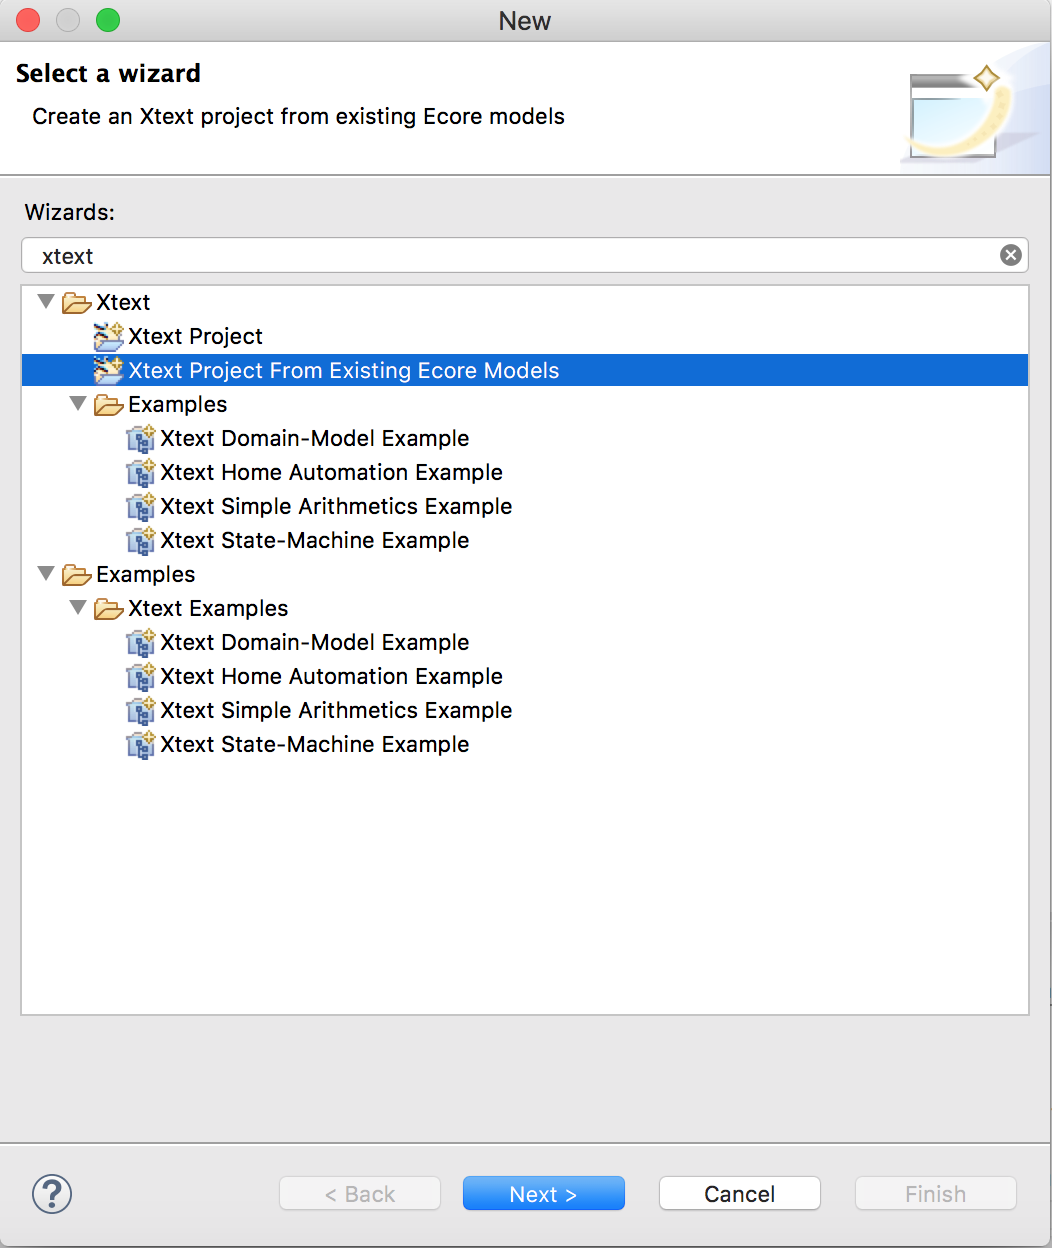
\includegraphics[scale=0.4]{images/emf_capturas/xtext-desde-ecore-paso1}
    \sourcepropia{}
    \caption{Creación de un proyecto Xtext desde un proyecto EMF ecore.}
    \label{fig:xtext_desde_ecore1}
\end{figure}
\begin{figure}
	\centering
    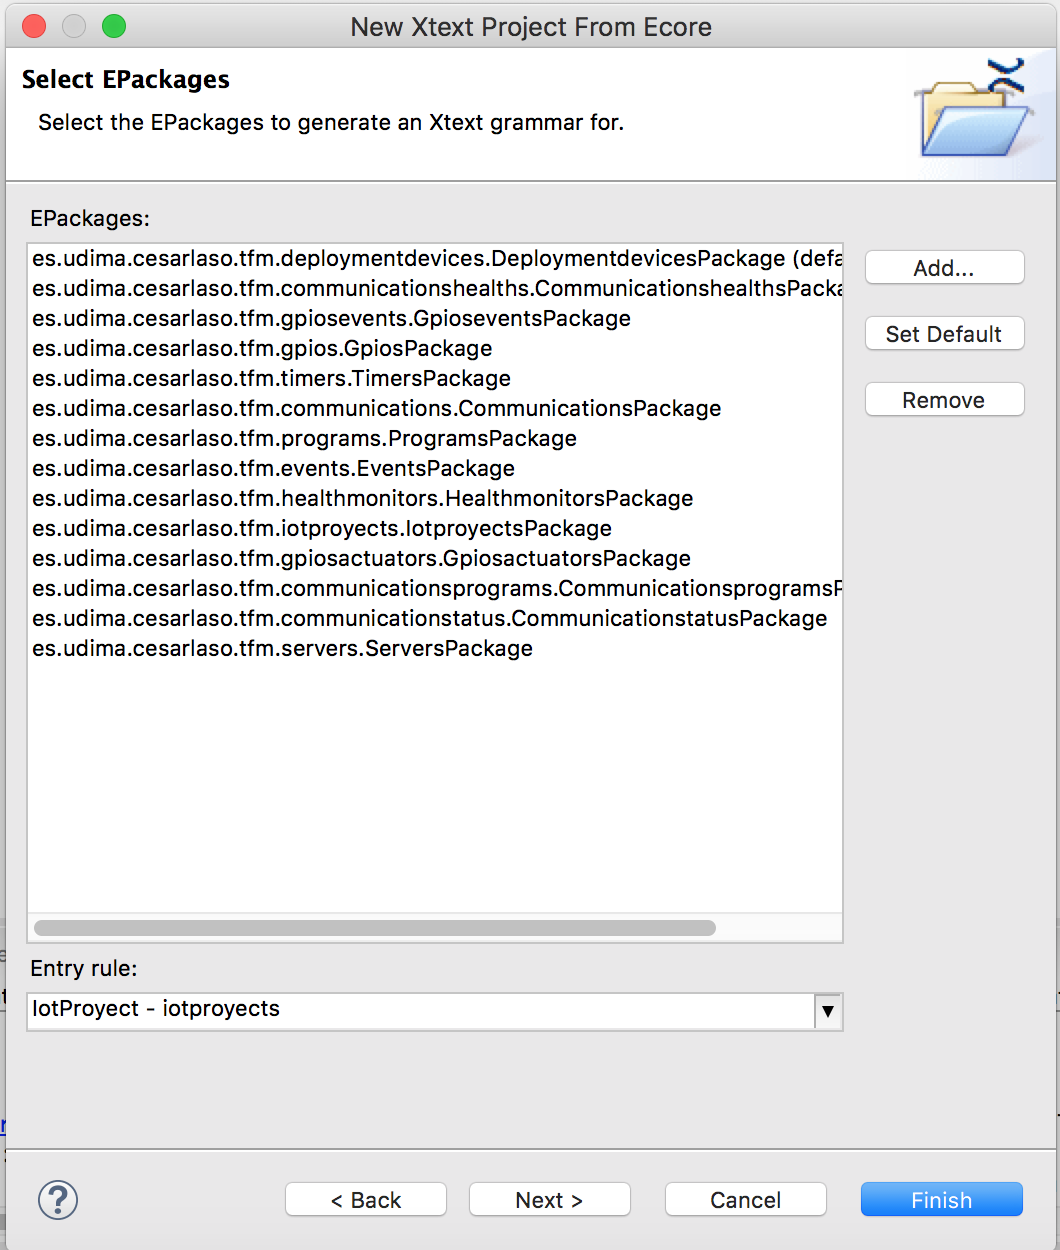
\includegraphics[scale=0.4]{images/emf_capturas/xtext-desde-ecore-paso2}
    \caption{Xtext en su importación desde \gls{ecore}. Selección de modelos que serán generados en la gramática y selección de elemento raíz.}
    \label{fig:xtext_desde_ecore2}
\end{figure}
\begin{figure}
	\centering
    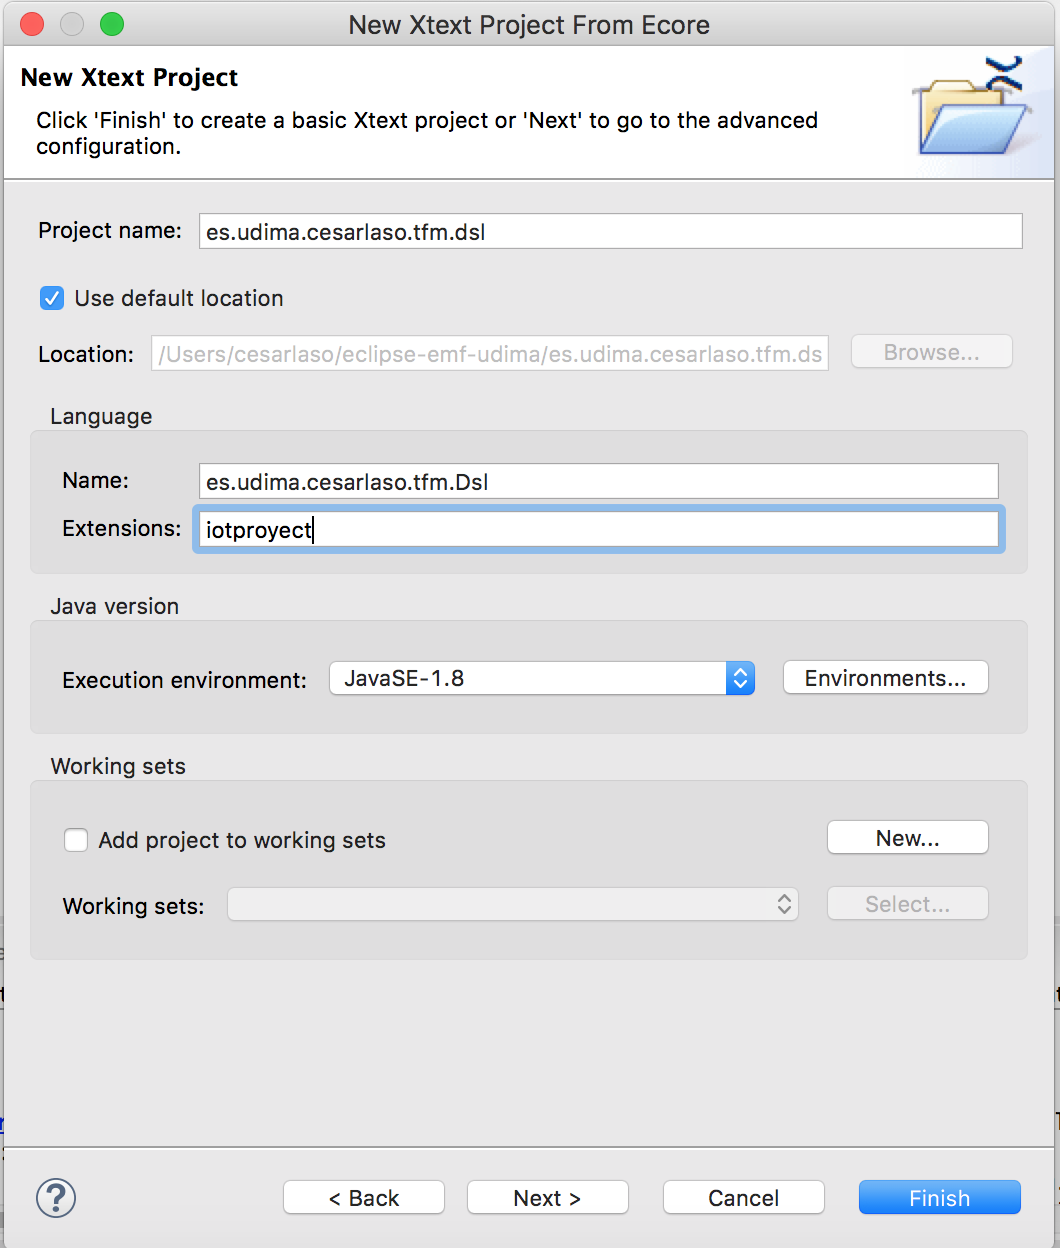
\includegraphics[scale=0.4]{images/emf_capturas/xtext-desde-ecore-paso3.png}
    \sourcepropia{}
    \caption{Nombre de nuestro DSL y extensión de archivo para el editor Eclipse EMF.}
    \label{fig:xtext_desde_ecore3}
\end{figure}


\subsection{Gramática}

La figura \ref{fig:xtext_dsl_definicio_ejemplo} muestra un listado ejemplo de definición de un evento. En este caso el evento \textit{analog read on high} que como el nombre indica, aplicara un evento cuando lea un valor desde un pin analógico y su valor sea mayor que un valor dado, consultando dicho estado cada x iteraciones o loops.

\begin{figure}
	\centering

\begin{lstlisting}

GpioAnalogReadPerformOnHigh returns gpiosevents::AnalogReadPerformOnHigh:
	'analog_read_on_high'
	pin=[gpios::AnalogPin|EString]
	'every' pollIntervalLoops=EInt 'loops'
	'value_higher_than' value=EInt
	'{' actuators+=Actuator ( "," actuators+=Actuator)* '}'
;

\end{lstlisting}
\sourcepropia{}
\caption{DSL - Ejemplo de gramática para un evento}
\label{fig:xtext_dsl_definicio_ejemplo}
\end{figure}

Puede consultarse la definición completa del lenguaje creado en este proyecto en el anexo \ref{appendix:dsl_final}.


\subsection{Ejemplos de programas}

\gls{xtext} proporciona al usuario final desarrollador del proyecto, un editor textual con soporte de auto completado. Al ser nuestro \gls{dsl} fuertemente tipado y específico al dominio, nos evita cometer errores ya no solo en tipos sino en estructura.

La figura \ref{fig:dsl_autocompletado_1} muestra la sección de programa, el auto completado solo permite que se añadan secciones que hereden del modelo Evento, ya sean estas de tipo \gls{gpio}, eventos de red, o eventos de tiempo. Si introdujéramos otro elemento de la gramática, el editor mostraría un error de compilación.

\begin{figure}
	\centering
    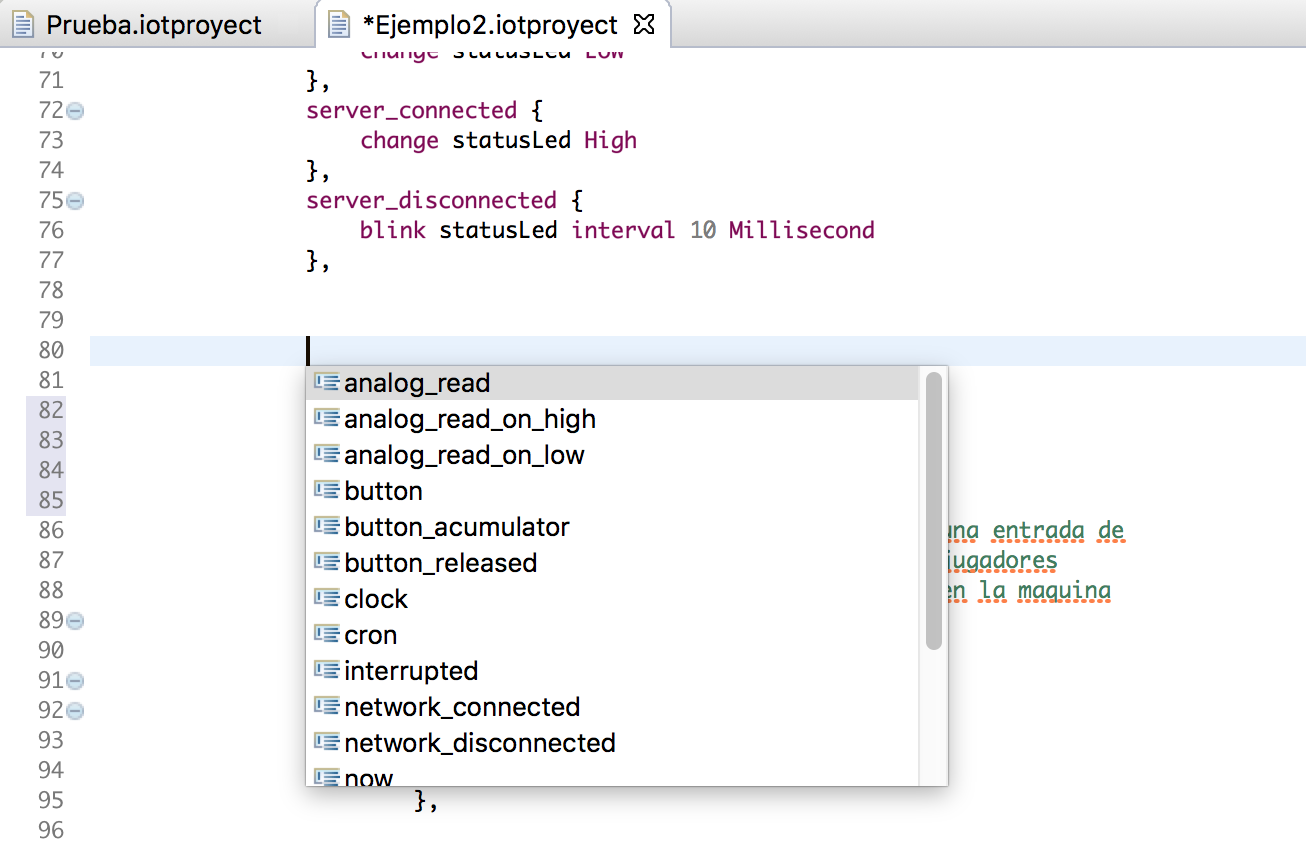
\includegraphics[scale=0.4]{images/emf_capturas/autocompletado_dsl_1.png}
    \sourcepropia{}
    \caption{Editor DSL. Autocompletado con modelos que implementen eventos.}
    \label{fig:dsl_autocompletado_1}
\end{figure}

A continuación podemos ver en la figura \ref{fig:dsl_autocompletado_2} como al especificar un elemento de tipo evento \gls{gpio}, el auto completado rellena la selección solamente con las variables anteriormente definidas, estas de tipo \textit{GpioInput}, no permitiendo especificar variables de tipo salida en una entrada, o variables de tipo de digital en una analógica.

\begin{figure}
	\centering
    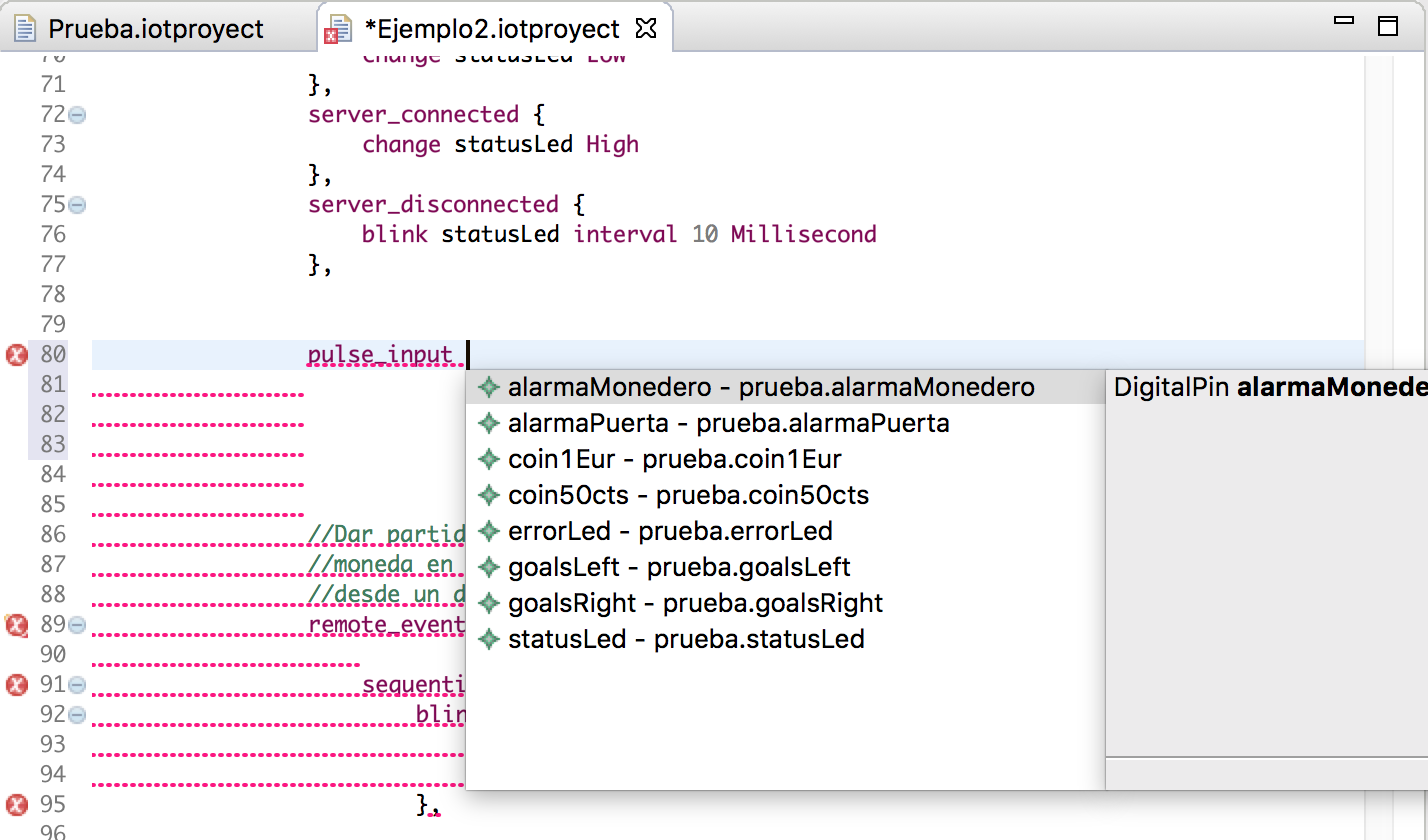
\includegraphics[scale=0.4]{images/emf_capturas/autocompletado_dsl_2.png}
    \caption[Editor DSL - Restricción en variables]{Editor DSL. El editor DSL solo permitirá utilizar las variables previamente definidas y permitidas para el tipo de evento definido en la gramática.}
    \label{fig:dsl_autocompletado_2}
\end{figure}

En la figura \ref{fig:dsl_autocompletado_3} vemos como el auto completado y restricción de la gramática permite no solo definir elementos globales sino incluso definir elementos dentro de elementos, en este caso, una entrada de pulso asociado a una variable ya existente, solo podrá contener dos modos válidos de interrupción.

\begin{figure}
	\centering
    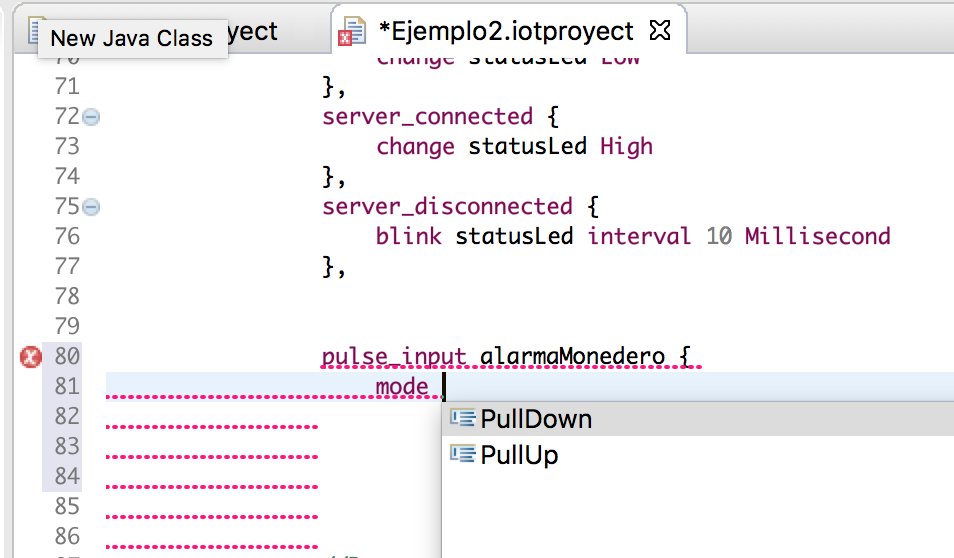
\includegraphics[scale=0.4]{images/emf_capturas/autocompletado_dsl_3.png}
    \sourcepropia{}
    \caption[Editor DSL - Tipado en atributos]{Edición de programa DSL, los atributos están fuertemente tipados también en valor.}
    \label{fig:dsl_autocompletado_3}
\end{figure}

Por último, podemos ver en la figura \ref{fig:dsl_autocompletado_4}  como el editor nos auto completa con los elementos ya referenciados. En el caso de definir un actuador para un evento, el editor muestra todas las reglas gramaticales válidas para un actuador, del tipo que sea, incluso un grupo de actuadores secuenciales donde incluir a su vez otros actuadores.

\begin{figure}
	\centering
    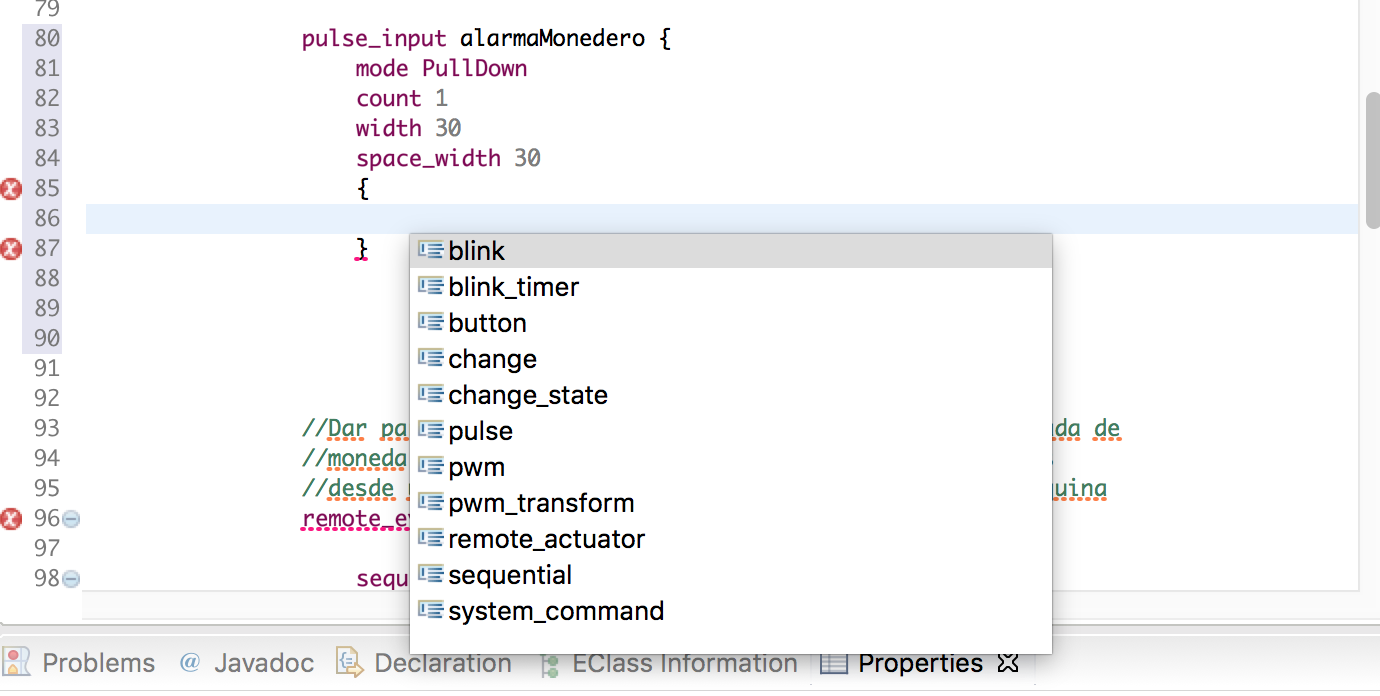
\includegraphics[scale=0.4]{images/emf_capturas/autocompletado_dsl_4.png}
    \sourcepropia{}
    \caption[Editor DSL - Autocompletado de variables]{Edición de programa DSL, al crear nuevos actuadores, nos muestra selección de los existentes.}
    \label{fig:dsl_autocompletado_4}
\end{figure}
